\documentclass[a4paper,10pt]{article}

%Packages
\usepackage{txfonts}
\usepackage{titlesec}
\usepackage[utf8]{inputenc}
\usepackage[T1]{fontenc}
\usepackage{geometry}
\usepackage{graphicx}
\usepackage{multicol}
\usepackage{fancyhdr}
\usepackage{hyperref}
\usepackage{float}
\usepackage{setspace}
\usepackage{caption}
\usepackage{booktabs}

% PAGE LAYOUT
\geometry{a4paper, top=18mm, bottom=18mm, textwidth=185mm}
\setlength{\columnsep}{6mm}
\setlength{\parindent}{0pt}

\titleformat{\section}
{\normalfont\bfseries}
	{\thesection.}{0.5em}{}
\titleformat{\subsection}
	{\normalfont\itshape}
	{\thesubsection.}{0.5em}{}

\pagestyle{fancy}
\renewcommand{\footrulewidth}{0pt}
\fancyhf{}
\rhead{
\includegraphics[scale=0.4]{Images/hepia_simple.png}}
\rfoot{\textit{\today}}
\cfoot{\thepage}

\captionsetup{
  font=footnotesize,
  labelsep=colon
}

\begin{document}

\begin{multicols*}{2}
[
\begin{center}
\vspace*{0mm}
{\large
AI in Healthcare – Data Preparation and Analysis \\
\vspace{3mm}
Data Preparation, Summarization, Visualization, Reduction and \\
Diagnostic Performance Analysis of a Prostate Cancer Cohort
}\\
\vspace{8mm}
Guilhem Rozier Vilardell\footnote{\textit{\href{mailto:guroz26@student.sdu.dk}{guroz26@student.sdu.dk}}}
\\
\vspace{3mm}
\footnotesize{
\textit{AI in Healthcare Summer Camp – Data Preparation, Summarization, Visualization and Reduction}
}\\
\vspace{9mm}
\end{center}
\rule{\linewidth}{0.4pt}
\onehalfspacing
\textbf{Abstract}\\
Three raw datasets (demographic/clinical, biochemical, comorbidity codes) were cleaned, merged and imputed into a single table (1,159 patients, 25 variables). PSA was evaluated as a metastasis marker via ROC (AUC=0.670). PCA reduced ten biochemical markers to three components (69.3\% variance). A logistic regression model with backward elimination and 10-fold cross-validation reached AUC 0.855 (accuracy 0.783), outperforming PSA alone. SVM and random forest performed similarly. LIME explained one patient's prediction. PSA alone is a moderate discriminator; combining biomarkers, comorbidities and demographics improves prediction substantially.\\
\noindent\textit{Keywords:} prostate cancer, PSA, ROC, PCA, logistic regression, cross-validation, LIME\\
\rule{\linewidth}{0.4pt}
]
\singlespacing

\tableofcontents

\setlength{\parskip}{1pt}
\columnbreak

\section{Introduction}
Prostate cancer (PC) is common and diagnosis relies on heterogeneous data: clinical records, laboratory tests, and medical history. Before modelling, data must be cleaned and merged. This report covers data preparation, visualisation, feature reduction and classification. The main questions: (i) how to prepare three separate sources into one reliable table, and (ii) how well does PSA alone discriminate metastasis, and can the biomarker panel be compressed without losing too much information.

\section{Data}
Three source files, linked by patient \texttt{ID}:
\begin{itemize}
\item \textbf{DATASET1} – clinical: civil status, family cancer history, metastasis (outcome), dates (diagnosis, metastasis, birth).
\item \textbf{DATASET2} – laboratory: ten numeric markers (monocyte, urea, lymphocyte, thrombocyte, erythrocyte, albumin, creatinine, globulin, PSA, coagulation factor).
\item \textbf{DATASET3} – medical history: one row per condition (diabetes, hearing loss, hypercholesterolaemia, hypertension, osteoporosis, urinary retention).
\end{itemize}

\section{Data Preparation and Results}

\subsection{Type correction and reshaping}
\textbf{Method:} Converted categorical variables in DATASET1 to proper types; parsed dates. DATASET2 types were already correct. DATASET3 was pivoted from long to wide format, creating one binary column per disease.

\textbf{Result:} All variables now in correct format for analysis.

\subsection{Missing data and imputation}
\textbf{Method:} Checked missingness. DATASET1 had 63.7\% missing in metastasis date (expected for non-metastatic patients). DATASET2 had scattered missingness (0.3–14.1\%). Histograms (Fig.~\ref{fig:hist}) showed most markers skewed, so we used median imputation (robust to outliers).

\textbf{Result:} Missing data handled; no patient loss.

\begin{figure}[H]
\centering
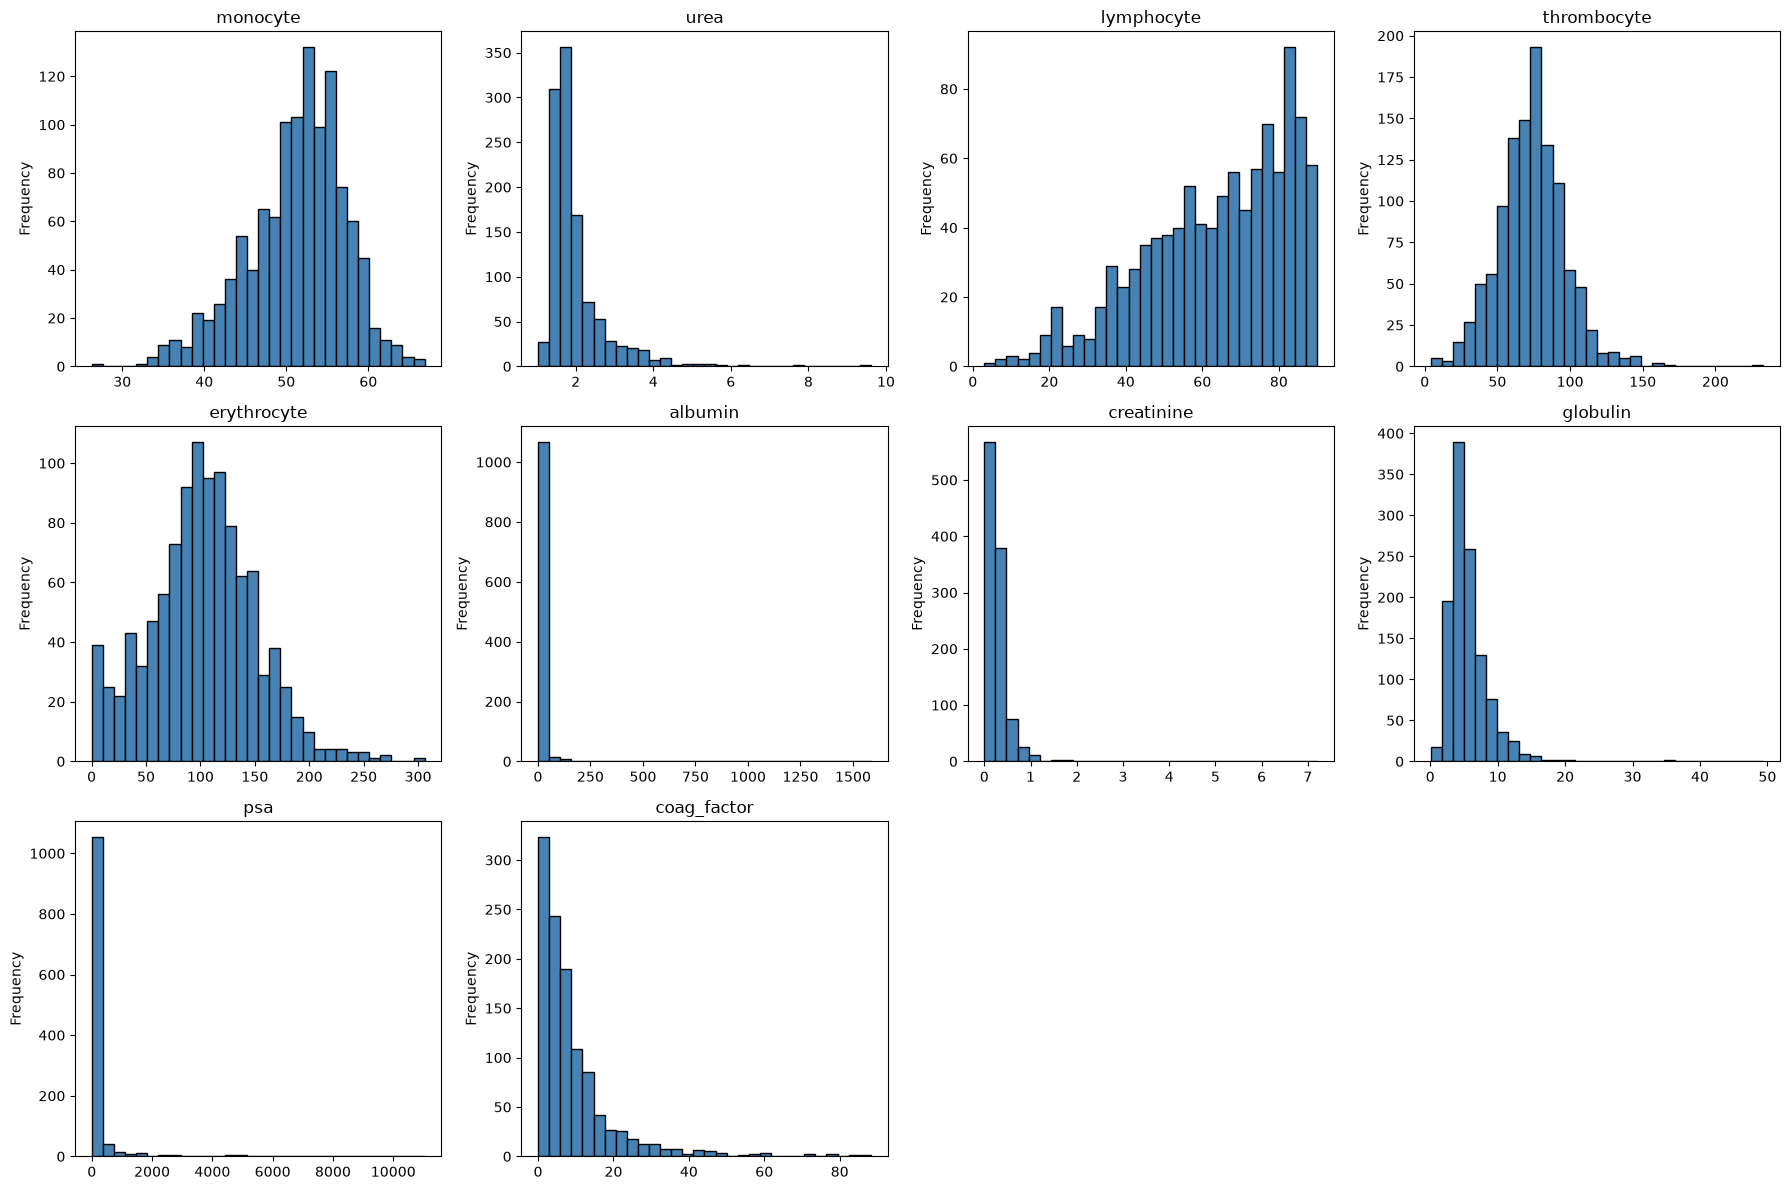
\includegraphics[width=\linewidth]{Images/biomarker_hist.png}
\caption{Distributions of ten biochemical markers.}
\label{fig:hist}
\end{figure}

\subsection{Merging}
\textbf{Method:} Left-joined DATASET1, DATASET2 and the wide disease table on \texttt{ID}. Missing disease flags set to 0.

\textbf{Result:} Final merged dataset \texttt{DATASET123}: 1,159 rows × 25 columns.

\subsection{Patient characteristics}
Table~\ref{tab:characteristics} summarises the cohort.

\begin{table}[H]
\centering
\caption{Patient characteristics (N=1,159).}
\label{tab:characteristics}
\begin{tabular}{lr}
\toprule
Variable & Value \\
\midrule
Age at PC diagnosis (yr) & 74.3 $\pm$ 8.7 \\
Age at metastasis (yr)$^{*}$ & 78.9 $\pm$ 8.5 \\
Metastasis: yes & 421 (36.3\%) \\
Family history: yes & 623 (53.8\%) \\
Civil status: married/cohabiting & 808 (69.7\%) \\
\bottomrule
\end{tabular}\\
\footnotesize{$^{*}$only for patients with metastasis.}
\end{table}

About one third developed metastasis, on average 4.6 years after diagnosis.
\columnbreak
\subsection{Correlation structure}
\textbf{Method:} Computed Pearson correlations among the ten biomarkers and visualised as heatmap (Fig.~\ref{fig:corr}).

\textbf{Result:} Most correlations weak; no strong collinearity. All markers can be used.

\begin{figure}[H]
\centering
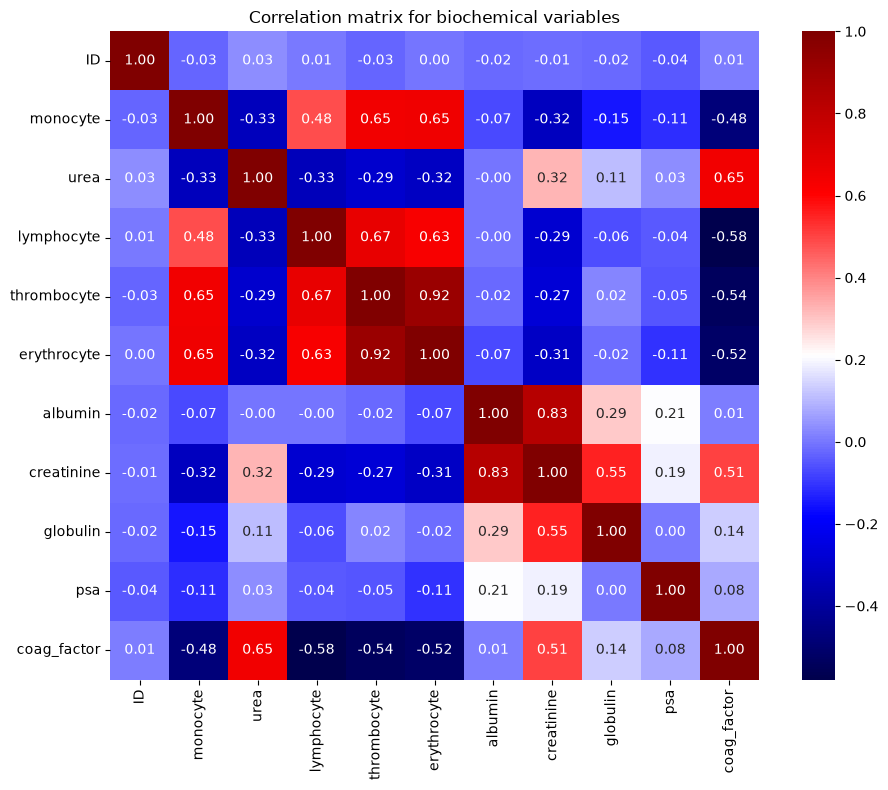
\includegraphics[width=\linewidth]{Images/corr_heatmap.png}
\caption{Correlation matrix of biochemical markers.}
\label{fig:corr}
\end{figure}

\subsection{PSA diagnostic performance}
\textbf{Method:} Tested two fixed cutoffs (20 and 100 ng/mL) for metastasis classification; performed ROC analysis and determined optimal cutoffs via Youden index and maximum accuracy.

\textbf{Result:} Table~\ref{tab:psa} shows performance. Lower cutoff gives higher sensitivity; higher cutoff gives higher specificity. Accuracy similar (~0.65) due to class imbalance.

\begin{table}[H]
\centering
\caption{PSA performance at fixed cutoffs.}
\label{tab:psa}
\begin{tabular}{lcc}
\toprule
 & PSA $>$20 & PSA $>$100 \\
\midrule
Sensitivity & 0.596 & 0.323 \\
Specificity & 0.672 & 0.867 \\
Accuracy & 0.645 & 0.670 \\
\bottomrule
\end{tabular}
\end{table}

ROC curve (Fig.~\ref{fig:roc}) gave AUC = 0.670 – moderate discrimination. Youden index chose 23 ng/mL; max accuracy chose 134 ng/mL.

\begin{figure}[H]
\centering
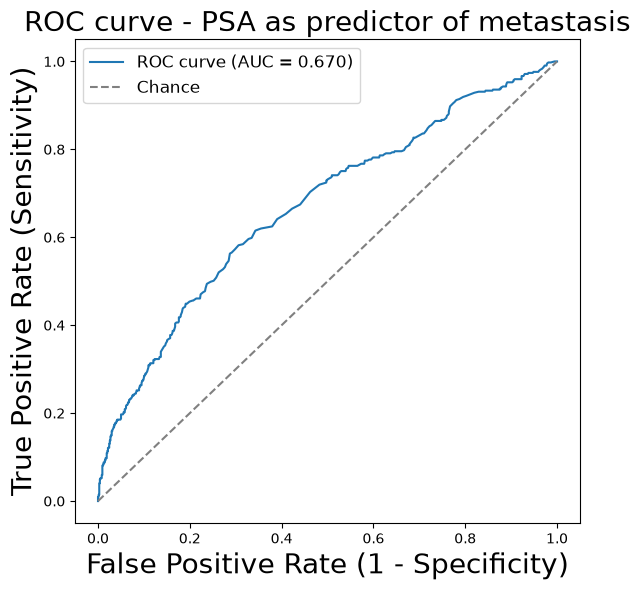
\includegraphics[width=\linewidth]{Images/roc_curve.png}
\caption{ROC curve for PSA (AUC=0.670).}
\label{fig:roc}
\end{figure}

\subsection{Principal Component Analysis (PCA)}
\textbf{Method:} Standardised biomarkers and performed PCA. Retained components with eigenvalue $>1$ (Kaiser criterion).

\textbf{Result:} Three components retained (eigenvalues 3.90, 1.95, 1.10), explaining 69.3\% of variance (Fig.~\ref{fig:scree}). Loadings in Table~\ref{tab:loadings}. PC1: cellular markers, PC2: renal/nutritional, PC3: PSA-dominated. Good dimensionality reduction.

\begin{figure}[H]
\centering
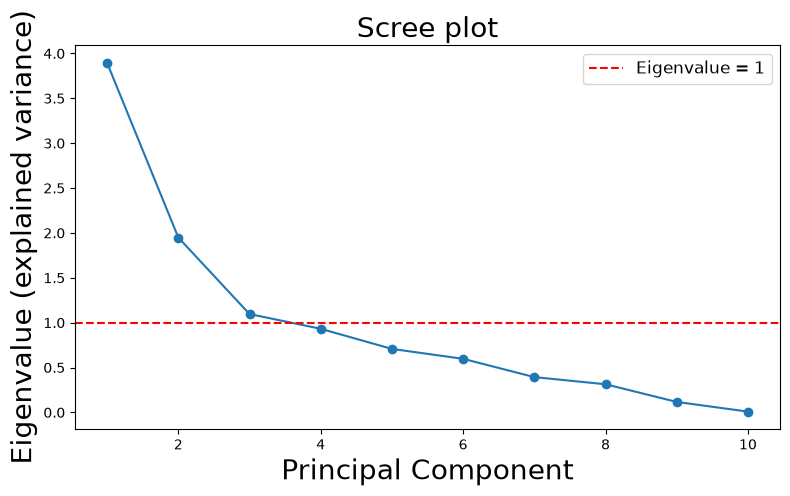
\includegraphics[width=\linewidth]{Images/scree_plot.png}
\caption{Scree plot with Kaiser cutoff.}
\label{fig:scree}
\end{figure}

\begin{table}[H]
\centering
\caption{PCA loadings (top per component).}
\label{tab:loadings}
\begin{tabular}{lrrr}
\toprule
Marker & PC1 & PC2 & PC3 \\
\midrule
monocyte     & 0.381  & 0.112  & -0.137 \\
urea         & -0.290 & -0.041 & -0.479 \\
lymphocyte   & 0.348  & 0.167  & 0.051 \\
thrombocyte  & 0.412  & 0.245  & -0.225 \\
erythrocyte  & 0.412  & 0.199  & -0.260 \\
albumin      & -0.132 & 0.593  & 0.248 \\
creatinine   & -0.323 & 0.532  & -0.047 \\
globulin     & -0.128 & 0.436  & -0.345 \\
psa          & -0.085 & 0.173  & 0.600 \\
coag\_factor & -0.405 & -0.063 & -0.296 \\
\bottomrule
\end{tabular}
\end{table}

\subsection{Univariate logistic regression (urinary retention)}
\textbf{Method:} Fitted simple logistic regression: metastasis $\sim$ urinary\_retention.

\textbf{Result:} Significant (OR=2.49, p<0.001) but low $R^2=0.029$. Accuracy at 0.5 cutoff: 65\%, recall 37\%.

\subsection{Multiple logistic regression and collinearity}
\textbf{Method:} Full model with all 21 predictors (excluding ID, dates, PCA components). Checked VIF.

\textbf{Result:} Pseudo $R^2=0.320$. High VIF for creatinine, albumin, coagulation factor (Table~\ref{tab:vif}) – collinearity issue. Replacing biomarkers with PC1-3 solved VIF.

\begin{table}[H]
\centering
\caption{VIF values (raw biomarkers).}
\label{tab:vif}
\begin{tabular}{lr}
\toprule
Variable & VIF \\
\midrule
Creatinine & 63.4 \\
Albumin & 35.4 \\
Coagulation factor & 14.7 \\
Globulin & 6.6 \\
Thrombocyte & 5.3 \\
\bottomrule
\end{tabular}
\end{table}

\subsection{Backward elimination}
\textbf{Method:} Removed predictors one by one based on p-value until all remaining significant ($\alpha=0.05$).

\textbf{Result:} Dropped 8 variables (including creatinine and coagulation factor). Final model had 13 predictors, AIC improved. In-sample performance at 0.5 cutoff: accuracy 0.79, recall 0.68, precision 0.72 (Table~\ref{tab:final_perf}).

\begin{table}[H]
\centering
\caption{Final model in-sample performance.}
\label{tab:final_perf}
\begin{tabular}{lccc}
\toprule
Class & Precision & Recall & F1 \\
\midrule
No metastasis & 0.82 & 0.85 & 0.84 \\
Metastasis & 0.72 & 0.68 & 0.70 \\
\midrule
Accuracy & \multicolumn{3}{c}{0.79} \\
\bottomrule
\end{tabular}
\end{table}

\subsection{Cross-validated performance}
\textbf{Method:} 10-fold stratified cross-validation on final model.

\textbf{Result:} Mean metrics: accuracy 0.783 (SD 0.028), sensitivity 0.675 (SD 0.058), specificity 0.846, precision 0.718, F1 0.693, AUC 0.855 (SD 0.023). Stable. Huge improvement over PSA alone (AUC +0.185).

\subsection{Model comparison}
\textbf{Method:} Compared logistic regression, SVM, random forest, L1-logistic via same CV.

\textbf{Result:} All performed similarly (Table~\ref{tab:modelcomp}). Logistic regression has interpretable coefficients, so preferred.

\begin{table}[H]
\centering
\caption{Cross-validated performance by model.}
\label{tab:modelcomp}
\begin{tabular}{lccccc}
\toprule
Model & Acc. & Sens. & Prec. & F1 & AUC \\
\midrule
Logistic Reg. & 0.783 & 0.675 & 0.718 & 0.693 & 0.855 \\
SVM & 0.786 & 0.713 & 0.705 & 0.707 & 0.841 \\
Random Forest & 0.785 & 0.682 & 0.716 & 0.696 & 0.843 \\
Reg. LR (L1) & 0.783 & 0.677 & 0.717 & 0.694 & 0.855 \\
\bottomrule
\end{tabular}
\end{table}

\subsection{LIME explanation}
\textbf{Method:} Used LIME on one random patient to explain prediction.

\textbf{Result:} Top influential features: family history, albumin, diabetes, age, lymphocytes. LIME shows direction of each contribution for that patient.

\section{Conclusion}
\textbf{Interpretation:} We produced a clean merged dataset. PSA alone is a moderate discriminator (AUC 0.670), no single cutoff is perfect. PCA reduces ten markers to three components retaining 69\% variance. A multivariable logistic model (13 predictors, cross-validated AUC 0.855) beats PSA significantly and remains interpretable. SVM and random forest give similar performance but are less transparent.

\textbf{Impact:} The logistic model can support risk stratification. The ROC analysis provides data-driven cutoffs when only PSA is available.

\textbf{Limitations:} Retrospective, cross-sectional design limits causal claims. Issues: median imputation should be verified; PSA>20 flag duplicates continuous PSA; diabetes coefficient negative (unexpected) – needs expert review. Future prospective studies with time-to-event data could use survival analysis.

\end{multicols*}
\section{Annexe}
\begin{figure}[H]
\centering
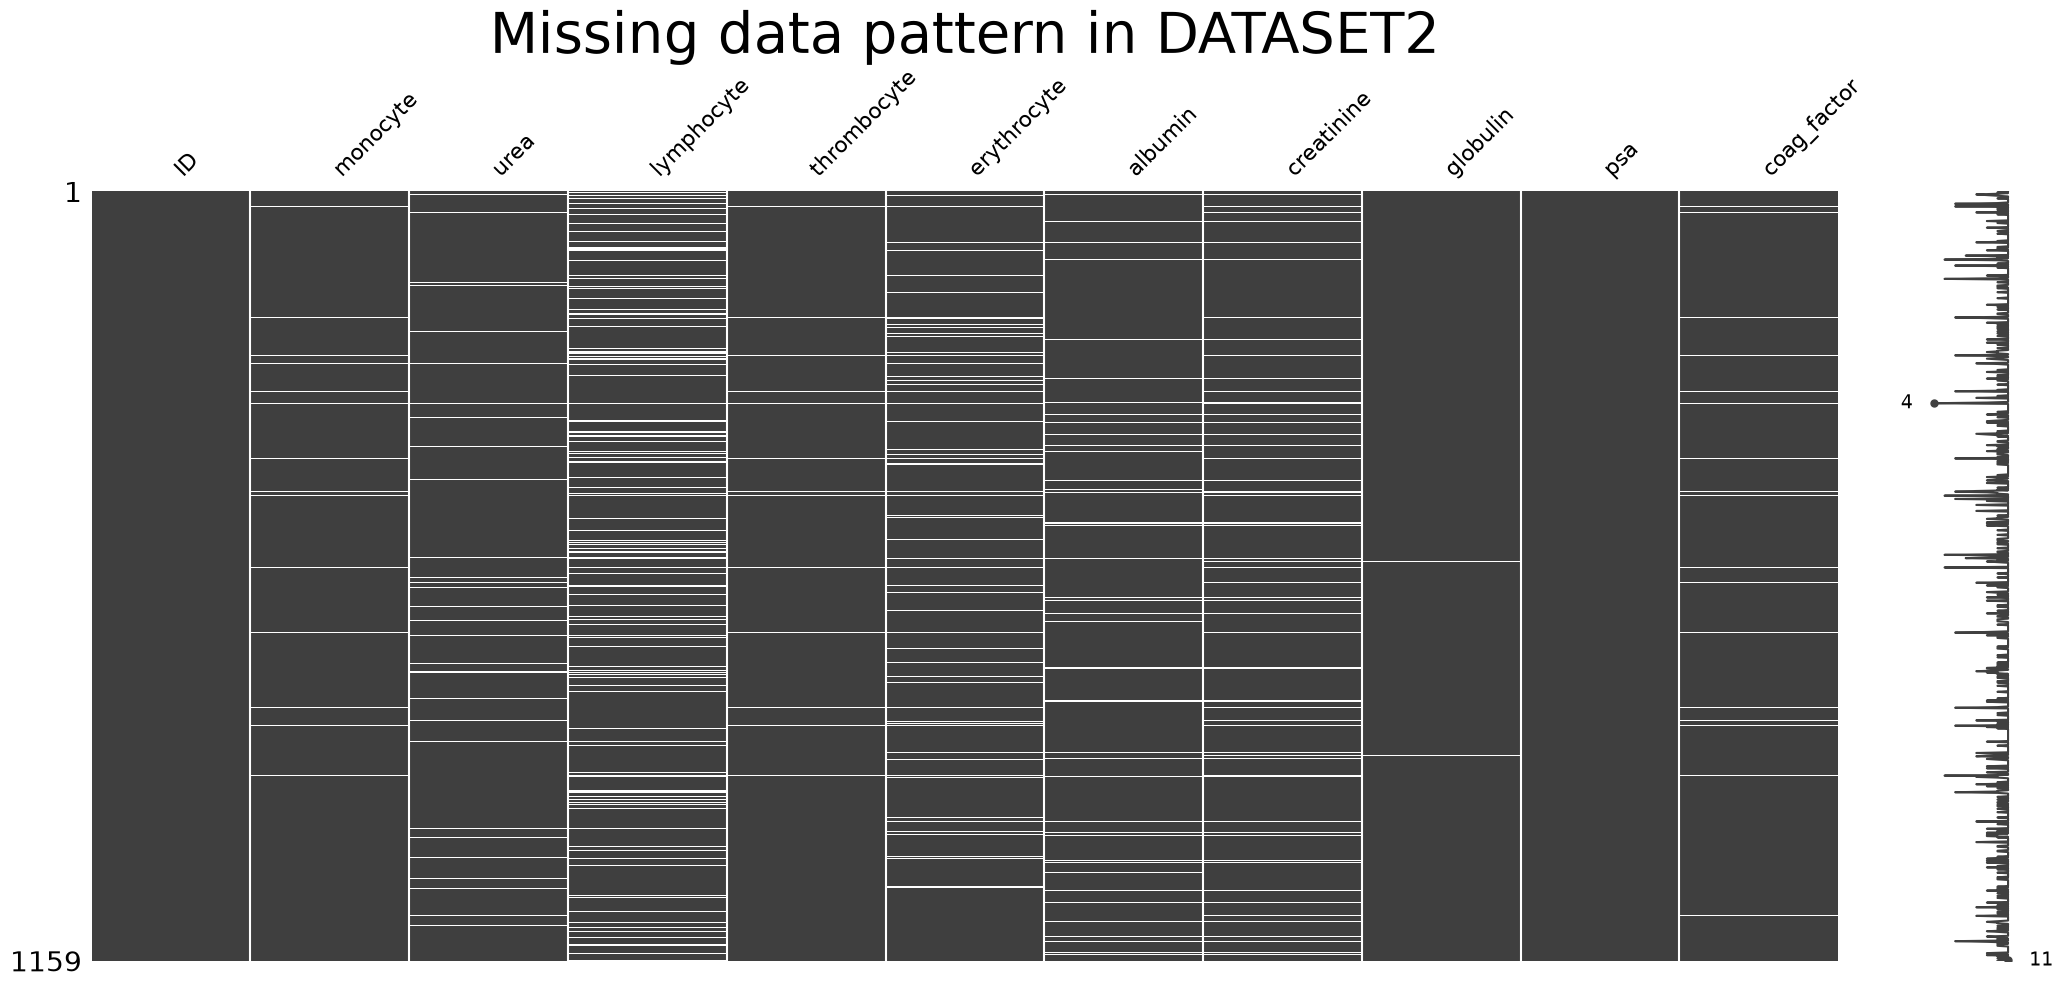
\includegraphics[width=\linewidth]{Images/missing_matrix.png}
\caption{Missingness pattern in DATASET2 (scattered).}
\label{fig:missmat}
\end{figure}
\end{document}